\section{Écrire des mathématiques}

\begin{frame}{Packages minimum utiles}
    \begin{itemize}[label=$\triangleright$]
        \item \texttt{amsfonts}
        \item \texttt{amsmath}
        \item \texttt{amssymb}
        \item \texttt{amsthm}
    \end{itemize}
\end{frame}

\begin{frame}[containsverbatim]
    \frametitle{Environnements différents}
    \begin{exampleblock}{En ligne}
        Savez-vous que $\pi=3.14$ ?
    \end{exampleblock}
    \begin{lstlisting}[language=TeX]
        Savez-vous que $\pi=3.14$ ?
    \end{lstlisting}
    \bigskip
    \begin{exampleblock}{Hors-ligne}
        Savez-vous que \[ \pi=3.14 \] ?
    \end{exampleblock}
    \begin{lstlisting}[language=TeX]
        Savez-vous que \[ \pi=3.14 \] ?
    \end{lstlisting}
\end{frame}

\begin{frame}[containsverbatim]
    \frametitle{Équations hors-ligne}
    \begin{exampleblock}{Numérotée}
        L'équation de l'Univers est :
        \begin{equation}
            e = m\cdot c^2
        \end{equation}
    \end{exampleblock}
    \begin{lstlisting}[language=TeX]
        L'equation de l'Univers est :
        \begin{equation}
            e = m \cdot c^2
        \end{equation}
    \end{lstlisting}
    \bigskip
\end{frame}

\begin{frame}[containsverbatim]
    \frametitle{Équations hors-ligne}
    \begin{exampleblock}{Non numérotée}
        L'équation de l'Univers est :
        \begin{equation*}
            e = m\cdot c^2
        \end{equation*}
    \end{exampleblock}
    \begin{lstlisting}[language=TeX]
    L'equation de l'Univers est :
    \begin{equation*}
    e = m \cdot c^2
    \end{equation*}
    \end{lstlisting}
    \bigskip
\end{frame}

\begin{frame}[containsverbatim]
    \frametitle{Exemples d'équations}
    \begin{columns}
        \column{0.3\textwidth}
        \begin{align*}
            m &= \cfrac{e}{c^{2}} \\
            c &= \pm \sqrt{\cfrac{e}{m}}
        \end{align*}
        \begin{equation*}
            \sin^2 x + \cos^2 x = 1
        \end{equation*}
        \begin{align*}
            \displaystyle{\int_3^{6x} x^3 + \sin^2 dx} \\ 
            \displaystyle{\mathbf{\mu_{Y}} \approx \mathbf{f(x)} + \cfrac{\partial \mathbf{f}}{\partial \mathbf{x}} \cdot \Delta \mathbf{x}}
        \end{align*}
        \column{0.7\textwidth}
        \footnotesize
        \begin{lstlisting}[language=TeX]
        \begin{align*}
        m &= \cfrac{e}{c^{2}} \\
        c &= \pm \sqrt{ \cfrac{e}{m} }
        \end{align*}
        \end{lstlisting}
        \begin{lstlisting}[language=TeX]
        \begin{equation*}
        \sin^2 x + \cos^2 x = 1
        \end{equation*}
        \end{lstlisting}
        \begin{lstlisting}[language=TeX]
        \begin{align*}
        \int_3^{6x} x^3 + \sin^2 dx \\ 
        \mathbf{\mu_{Y}} \approx 
        \mathbf{f(x)} + 
        \cfrac{\partial \mathbf{f}}
        {\partial \mathbf{x}} \cdot 
        \Delta \mathbf{x}
        \end{align*}
        \end{lstlisting}
    \end{columns}
\end{frame}

\begin{frame}[containsverbatim]
    \frametitle{Différentes matrices}
    \footnotesize
    \begin{table}
        \centering
        \begin{tabular}{ll}
            \verb|{matrix}|  & : matrice sans délimitateur    \\
            \verb|{pmatrix}| & : matrice entre parenthèses    \\
            \verb|{vmatrix}| & : matrice entre barres         \\
            \verb|{Vmatrix}| & : matrice entre doubles barres \\
            \verb|{bmatrix}| & : matrice entre croches        \\
            \verb|{Bmatrix}| & : matrice entre accolades      \\
        \end{tabular}
    \end{table}
    \begin{columns}
        \column{0.3\textwidth}
        \begin{center}
            $\begin{matrix} a&b \\ c&d \end{matrix} \qquad \begin{pmatrix} a&b \\ c&d \end{pmatrix}$
            $\begin{vmatrix} a&b \\ c&d \end{vmatrix} \qquad \begin{Vmatrix} a&b \\ c&d \end{Vmatrix}$
            $\begin{bmatrix} a&b \\ c&d \end{bmatrix} \qquad \begin{Bmatrix} a&b \\ c&d \end{Bmatrix}$
        \end{center}
        \column{0.7\textwidth}
        \verb|$\begin{matrix} a&b\\ c&d \end{matrix}$|   \\
        \verb|$\begin{pmatrix} a&b\\ c&d \end{pmatrix}$| \\
        \verb|$\begin{vmatrix} a&b\\ c&d \end{vmatrix}$| \\
        \verb|$\begin{Vmatrix} a&b\\ c&d \end{Vmatrix}$| \\
        \verb|$\begin{bmatrix} a&b\\ c&d \end{bmatrix}$| \\
        \verb|$\begin{Bmatrix} a&b\\ c&d \end{Bmatrix}$| \\
    \end{columns}
\end{frame}

\begin{frame}[containsverbatim]
    \frametitle{Divers symboles et polices}
    \begin{table}
        \centering
        \begin{tabular}{|c|l|l|}
            \hline
            $\mathrm{x=\sqrt{2}}$ & \verb|\mathrm{...}|     & romaine    \\ 
            \hline
            $\mathit{x=\sqrt{2}}$ & \verb|\mathit{...}|     & italique   \\
            \hline
            $\mathtt{x=\sqrt{2}}$ & \verb|\mathtt{...}|     & télétype   \\ 
            \hline
            $\mathbf{x=\sqrt{2}}$ & \verb|\mathbf{...}|     & gras       \\
            \hline
            $\mathsf{x=\sqrt{2}}$ & \verb|\mathsf{...}|     & sans-serif \\
            \hline
            $\mathbb{ABC}$        & \verb|\mathbb{ABC}|     & \\
            \hline
            $\mathcal{ABC}$       & \verb|\mathcal{ABC}|    & \\
            \hline
            $\mathscr{ABC}$       & \verb|\mathscr{ABC}|    & \\
            \hline
            $\mathfrak{ABC}$      & \verb|\mathfrak{ABC}|   & \\
            \hline
            $\mathnormal{ABC}$    & \verb|\mathnormal{ABC}| & \\
            \hline
        \end{tabular}
    \end{table}
\end{frame}

\begin{frame}[containsverbatim]
    \frametitle{Divers symboles et polices}
    \begin{table}
        \centering
        \begin{tabular}{|c|l|}
            \hline
            $\vec{x}$             & \verb|\vec{x}|             \\
            \hline
            $\overrightarrow{AB}$ & \verb|\overrightarrow{AB}| \\
            \hline
            $\cancel{x}$          & \verb|\cancel{x}|          \\
            \hline
            $\bcancel{x}$         & \verb|\bcancel{x}|         \\
            \hline
            $\xcancel{x}$         & \verb|\xcancel{x}|         \\
            \hline
        \end{tabular}
    \end{table}
    \begin{figure}
        \centering
        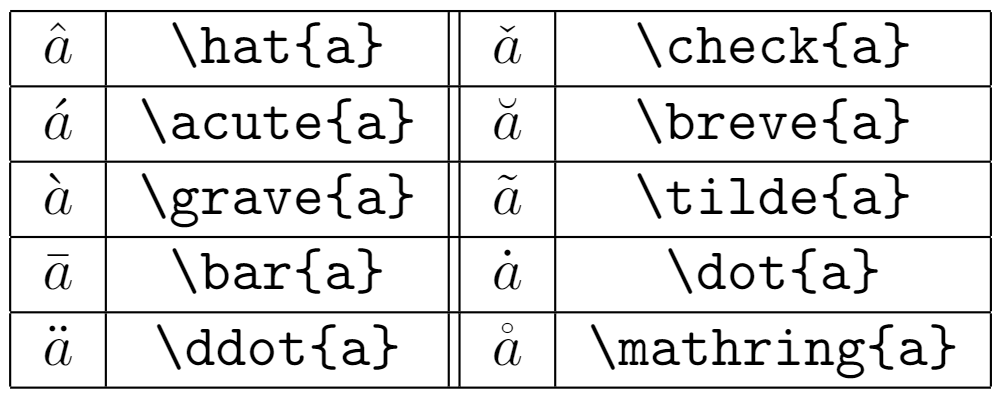
\includegraphics[width=7cm]{accentMathematiques.png}
    \end{figure}
\end{frame}

\begin{frame}[containsverbatim]
    \frametitle{Lettres grecques}
    \begin{table}
        \centering
        \begin{tabular}{|c|l||c|l||c|l|}
            \hline
            $\alpha$    & \verb|\alpha|    & $\beta$    & \verb|\beta|    & $\gamma$      & \verb|\gamma|      \\
            $\delta$    & \verb|\delta|    & $\epsilon$ & \verb|\epsilon| & $\varepsilon$ & \verb|\varepsilon| \\
            $\zeta$     & \verb|\zeta|     & $\eta$     & \verb|\eta|     & $\theta$      & \verb|\theta|      \\
            $\vartheta$ & \verb|\vartheta| & $\iota$    & \verb|\iota|    & $\kappa$      & \verb|\kappa|      \\
            $\lambda$   & \verb|\lambda|   & $\mu$      & \verb|\mu|      & $\nu$         & \verb|\nu|         \\
            $\xi$       & \verb|\xi|       & $\pi$      & \verb|\pi|      & $\varpi$      & \verb|\varpi|      \\
            $\rho$      & \verb|\rho|      & $\varrho$  & \verb|\varrho|  & $\sigma$      & \verb|\sigma|      \\
            $\varsigma$ & \verb|\varsigma| & $\tau$     & \verb|\tau|     & $\upsilon$    & \verb|\upsilon|    \\
            $\phi$      & \verb|\phi|      & $\varphi$  & \verb|\varphi|  & $\chi$        & \verb|\chi|        \\
            $\psi$      & \verb|\psi|      & $\omega$   & \verb|\omega|   &               &                    \\
            \hline
        \end{tabular}
    \end{table}
\end{frame}

\begin{frame}[containsverbatim]
    \frametitle{Lettres grecques}
    \begin{table}
        \centering
        \begin{tabular}{|c|l||c|l|}
            \hline
            $\Gamma$ & \verb|\Gamma| & $\Delta$   & \verb|\Delta|   \\
            $\Theta$ & \verb|\Theta| & $\Lambda$  & \verb|\Lambda|  \\
            $\Xi$    & \verb|\Xi|    & $\Pi$      & \verb|\Pi|      \\
            $\Sigma$ & \verb|\Sigma| & $\Upsilon$ & \verb|\Upsilon| \\
            $\Phi$   & \verb|\Phi|   & $\Psi$     & \verb|\Psi|     \\
            $\Omega$ & \verb|\Omega| &            &                 \\
            \hline
        \end{tabular}
    \end{table}
\end{frame}